\chapter{Evaluation}
\label{chap:eval}

In this chapter, we
evaluate the expressiveness
and performance of our API generation
toolchain.

%TODO: add when finalised
%with respect to the main objective
%of \dots

To evaluate the expressiveness
of our work,
we use two case studies
of protocols found in webservices
to demonstrate strengths and weaknesses
of our work:

\begin{itemize}

\item
\textbf{\tprotocol{Noughts and Crosses} Game:}

In \cref{section:evalgame},
we implement a classic multiplayer game which involves a game server
and two players interacting with the game via the browser,
to show that our work is compatible with multiparty sessions,
which isn't the case in \cite{MVU2020,Exceptional}.
We show how our generated APIs are compatible with the
state management solution used by the game, and give examples of 
how the generated APIs empower the developer to intuitively 
implement the game interface.

\item
\textbf{\tprotocol{Two Buyers} Protocol, as introduced in \cref{section:twobuyer}:}

In \cref{section:evaltwobuyer},
we walk through an implementation of the \tprotocol{Two Buyers}
protocol. This \textit{cannot} be implemented in
\cite{PureScript2019,MVU2020}, which illustrates the novelty
of our \newtheory theory on routed multiparty session types.
We emphasise how the routing mechanism is transparent to the
developer implementing the protocol, which demonstrates
the practicality of our extensions to \codegen to support
\newtheory.

\end{itemize}

To evaluate the performance of our work,
we run micro-benchmarks
on a variant of the \tprotocol{Ping Pong}
protocol parameterised by the number
of round trips
to analyse the overhead of our implementation,
compared with implementations written
without using our generated APIs,
as the number of round trips increase.
We describe the experiment methodology
and comment on our findings in \cref{section:benchmarks}.

\section{Multiparty Sessions: \tprotocol{Noughts and Crosses}}
\label{section:evalgame}

We implement the classic turn-based board game of \textit{Noughts and Crosses}
between two players,
as introduced in \cref{section:intro}.
We formalise the game interactions using a Scribble protocol
presented in \cref{lst:game}.
The \tprotocol{Game} protocol describes one turn:
\trole{P1} makes a move by sending the coordinates of a
vacant cell on the game board to \trole{Svr},
then \trole{Svr} reports the outcome of that move
to both players. If another round is required
to determine the game result, the \tprotocol{Game}
protocol is recursively invoked (\cref{line:gamerec}) with
roles \trole{P1} and \trole{P2} swapped.

\begin{figure}[!ht]
\begin{lstlisting}[language=Scribble]
module NoughtsAndCrosses;

// TypeScript definition:
// interface Point {x: number, y: number}
type <typescript> "Coordinate" from "./Types" as Point;

global protocol Game(role Svr, role P1, role P2) {
	Pos(Point) from P1 to Svr;
	choice at Svr {
		Lose(Point)   from Svr to P2;
		Win(Point)    from Svr to P1;
	} or {
		Draw(Point)   from Svr to P2;
		Draw(Point)   from Svr to P1;
	} or {
		Update(Point) from Svr to P2;
		Update(Point) from Svr to P1;
		do Game(Svr, P2, P1); (*@\label{line:gamerec}@*)
	}
}
\end{lstlisting}
\captionof{lstlisting}{The \tprotocol{Noughts and Crosses} Protocol}
\label{lst:game}
\end{figure}

We only highlight implementation details that
best illustrate the expressiveness of the generated APIs;
the interested reader should read the full implementation on
GitHub\footnote{
\url{https://github.com/ansonmiu0214/SessionTS-Examples/NoughtsAndCrosses}
}.

\subsection{Game Server}
We set up the WebSocket server as an Express.js \cite{Express} application
on top of the Node.js runtime.
We define our own game logic in a \texttt{Board} class
to keep track of the game state and expose methods 
to query the result.
This custom logic is integrated into the 
\texttt{handleP1Move} and \texttt{handleP2Move}
handlers implemented by the developer, defined to
handle the moves made by \trole{P1} and \trole{P2} respectively.
We illustrate this in \cref{lst:gamesvr}.

\begin{figure}[!h]
\begin{lstlisting}[language=javascript,tabsize=2]
const handleP1Move = new Implementation.S13({
	Pos: async (move: Point) => {
		// `board` manages game state;
		// `board.P1` registers the move and returns the game result
		const result = await board.P1(move);
		switch (result) {
			case MoveResult.Win: {
				return new Implementation.S15([
					// Send losing result to P2
					[Labels.S15.Lose, [move], new Implementation.S16(
						// Send winning result to P1
						[Labels.S16.Win, [move], new Implementation.Terminal()]
					)]
				]);
			}
			case MoveResult.Draw: { ... }
			case MoveResult.Continue: {
				return new Implementation.S15(
					// Notify both players and proceed
					// with next round using `handleP2Move`
					[Labels.S15.Update, [move], new Implementation.S18(
						[Labels.S18.Update, [move], handleP2Move]
					)]
				);	
			}		
		}
	}
});

const handleP2Move = ...		// Defined similarly as handleP1Move

new Svr(wss, handleP1Move, (role, reason) => {
	console.log(`${role} cancelled because of ${reason}`);
});
\end{lstlisting}
\captionof{lstlisting}{Implementing \tprotocol{Noughts and Crosses} Game Server using
\codegen}
\label{lst:gamesvr}
\end{figure}

When the server receives a move, it notifies
the game logic to update the game state and return the game
result caused by that move.
The game logic is likely to keep track of move history
using a database; we simulate this with a delay, so 
the game result returned by the game logic is a \texttt{Promise}.
The expressiveness of our generated APIs enable the developer
to define the handlers as \lstonelinejs{async} functions
to use the asynchronous game logic API intuitively -- this is something
prevalent in modern web programming, but not directly addressed in existing
session type implementations for web development \cite{PureScript2019,MVU2020}.

\subsection{Players}
For simplicity, our game uses the same implementation for both
\trole{P1} and \trole{P2}, although they can be different in theory --
the developer could implement \trole{P1} using a GUI and provide
\trole{P2} with a text-based game experience on the browser.

The main implementation detail for players
is to make a move. 
Intuitively, the developer implements a grid and binds a handler
to the \lstonelinejs{'onClick'} event of each vacant cell to send that cell's coordinate 
in a \tmsg{Pos(Point)} message to the game server.
A common source of bugs would be not preventing the user from selecting
a second cell when waiting for the game server's response,
which violates the game rules (and the global protocol).

Our approach of providing \textit{component factories} for send states
in \reactcodegen makes this very intuitive and guarantees communication safety.
First, it gives the developer the flexibility to trigger
the same send action (in this case, \tmsg{Pos(Point)} via multiple
UI elements -- the developer can generate a send action wrapper component 
for each vacant cell on the game board.
Moreover, each generated wrapper component sends a different payload
corresponding to the coordinates of the cell:
our generated APIs support this as the handler supplied
to the send component factory can access the cell's coordinates in the closure.
Finally, the send action is always followed by a transition to the receive
state component, so the user cannot violate channel linearity by selecting
two cells.

We demonstrate how this works in \cref{lst:gamesendfactory}.
The factory function for binding the \tmsg{Pos(Point)} send action
is defined under \lstonelinejs{this.props.Pos}.
For each x-y coordinate on the game board, if the cell is vacant,
we create a \texttt{<SelectPoint>} React component from the
component factory function (which reads ``build a react
component that sends the \tmsg{Pos} message with x-y coordinate
as payload when the user clicks on it''), and we wrap
a \texttt{<td>} table cell (since the game board is rendered as an
HTML table) inside the generated component to bind the click event
to the table cell.

\begin{figure}[!h]
\begin{lstlisting}[language=javascript,tabsize=2]
// Inside some render() function...
{board.map((row, x) =>
	<tr>
	{row.map((cell, y) => {
		if (cell === Cells.VACANT) {
			const sendPoint = (event: React.MouseEvent) => {
				// Don't refresh the screen
				event.preventDefault();
				return { x, y };
			});
			const SelectPoint = this.pros.Pos('onClick', sendPoint);
			return <SelectPoint><td>{cell}</td></SelectPoint>
		} else {
			// Render nought or cross,
			// but clicking on this cell 	will *not* send anything
			return <td>{cell}</td>
		}		
	})}
	</tr>
)}
\end{lstlisting}
\captionof{lstlisting}{\dots}
\label{lst:gamesendfactory}
\end{figure}

The developer can also leverage the session cancellation handler
to render useful messages to the player.
A different UI can be rendered depending on whether
the server or the opposition has disconnected,
and make \textit{application-specific} interpretations of the cancellation.
For example, if the opposition has disconnected,
the developer can interpret this as a forfeit and
render a winning message to the user.

\subsection{Summary}
We demonstrated how the developer can use the generated APIs
from \codegen to implement a complex multiparty protocol
which features branching, selection and recursion.
We highlighted specific features in the generated APIs for both
server and browser endpoints that allow the developer
to intuitively implement their application logic.
In particular, we observed that the extensions introduced
in \cref{chap:ext} played crucial roles in
improving the usability of the generated APIs.

\section{Routed Multiparty Sessions: \tprotocol{Two Buyers}}
\label{section:evaltwobuyer}

We implement the \tprotocol{Two Buyer} protocol
introduced in \cref{section:twobuyer}. 
This protocol cannot be implemented using
existing proposals \cite{PureScript2019,MVU2020} for integrating
session types into web development.
\codegen overcomes the limitations of existing work
through implementing novel theory of routed multiparty
session types formalised in \cref{chap:theory}.

We present the implementation of the \trole{S}eller
in \cref{lst:evaltwobuyerseller}, 
and the implementation
of the peer-to-peer interaction by buyer \trole{A}
in \cref{lst:evaltwobuyerA}
The main point to note is that the routing mechanism
is completely transparent to the developer,
which shows the elegance of our solution.

\begin{figure}[!h]
\begin{lstlisting}[language=javascript]
// two buyer seller
\end{lstlisting}
\captionof{lstlisting}{\dots}
\label{lst:evaltwobuyerseller}
\end{figure}

\begin{figure}[!h]
\begin{lstlisting}[language=javascript]
// two buyer A p2p
\end{lstlisting}
\captionof{lstlisting}{\dots}
\label{lst:evaltwobuyerA}
\end{figure}

The \newtheory implementation does not affect
the compatibility of our generated APIs with external libraries.
The \trole{S}eller endpoint is set up as an Express.js
application, and both buyers still use the React Context API
for application state management. We show an example of
the latter in the developer's implementation for
buyer \trole{A} receiving and keeping track of the server's quote
using a React Context in \cref{lst:evaltwobuyercontext}.

\begin{figure}[!h]
\begin{lstlisting}[language=javascript]
// two buyer A context
\end{lstlisting}
\captionof{lstlisting}{\dots}
\label{lst:evaltwobuyercontext}
\end{figure}

We include the implementations of the remaining EFSM states
for buyer \trole{A} in \cref{section:evalcodetwobuyer}
for completeness;
interested readers can find the full implementations for the other
endpoints alongside the generated code on
GitHub\footnote{
\url{https://github.com/ansonmiu0214/SessionTS-Examples/TwoBuyer}
}.


%\section{Delegated Sessions: \fancyname{ATM}}
\label{section:evalatm}

Interested readers can find the full implementation on
GitHub\footnote{\url{https://github.com/ansonmiu0214/SessionTS-Examples/ATM}}.

\begin{itemize}
\item Show that delegation is not supported
even if the protocol ``allows''
\end{itemize}

\begin{figure}[!ht]
\begin{lstlisting}[language=Scribble, tabsize=2]
module ATM;

global protocol ATM(role Bank, role Client) {
	choice at Client {
		// The string contains the client ID
		WITHDRAW(string, number) from Client to Bank;
		choice at Svr {
			BALANCE(number) from Bank to Client;		
		} or {
			FAIL(string) from Bank to Client;		
		}
		do ATM(Bank, Client);
	} or {
		DEPOSIT(string, number) from Client to Bank;
		BALANCE(number) from Bank to Client;
		do ATM(Bank, Client);
	} or {
		BYE(string) from Client to Bank;
		BYE() from Bank to Client;	
	}
}
\end{lstlisting}
\captionof{lstlisting}{The \tprotocol{ATM} Protocol}
\label{lst:atm}
\end{figure}
 

\section{Performance Benchmarks}

Whilst web applications that implement our generated APIs enjoy
communication safety guarantees, the presence of the session runtime acts
as an additional layer of abstraction between the application logic and the
WebSocket transport, which is likely to present a performance trade-off.

\begin{figure}[!ht]
\begin{lstlisting}[language=Scribble]
global protocol PingPong(role Client, role Svr) {
	PING(number) from Client to Svr;
	choice at Svr {
		PONG(number) from Svr to Client;
		do PingPong(Client, Svr);
	} or {
		BYE(number) from Svr to Client;	
	}
}
\end{lstlisting}
\captionof{lstlisting}{Ping Pong Protocol}
\label{lst:pingpong}
\end{figure}

To measure the overhead of our implementation, we compare the
execution time of an interactive web application implementing the
Ping Pong protocol (\cref{lst:pingpong}) using our generated APIs,
against implementations of the protocol \textit{without} session types.

We parameterise the Ping Pong protocol by $n > 0$, the number of
round-trip messages. This is standardised in the application logic
across experiments.
Upon establishing a connection, the experiment proceeds as follow:

\begin{enumerate}

\item \trole{Client} sends \tmsg{PING($m$:number)} to \trole{Svr}, 
with $m = 0$ initially.

\item \trole{Svr} receives \tmsg{PING($m$:number)}, and
conditionally responds based on $n$:

\begin{enumerate}
\item If $m + 1 < n$, then \trole{Svr} replies \tmsg{PONG($m + 1$)}.
\trole{Client} responds to \tmsg{PONG} by returning to
step 1 with $m$ set as the payload from \tmsg{PONG}.

\item Otherwise, $m + 1 = n$, then \trole{Svr} responds with 
\tmsg{BYE($m + 1$)}, as $n$ round trips have taken place. 
\trole{Client} responds to \tmsg{BYE} by 
closing the connection, thus ending the experiment.
\end{enumerate}

\end{enumerate}

We note that the Ping Pong protocol implements a \textit{binary} session. 
It would be interesting to observe the overhead in a \textit{multiparty}
context, but due to limited time constraints, we were unable to 
extend our benchmarking suite to support multiple browser targets.
Benchmarking multiparty protocols would also require writing multiple
distinct React applications using the generated APIs -- as this is currently
a manual process, doing this for multiple roles requires more time than
available.

\subsection{Setup}

In order to measure the overhead as accurately as possible,
we outline the logic that all implementations must follow:

\begin{figure}[!ht]
\centering
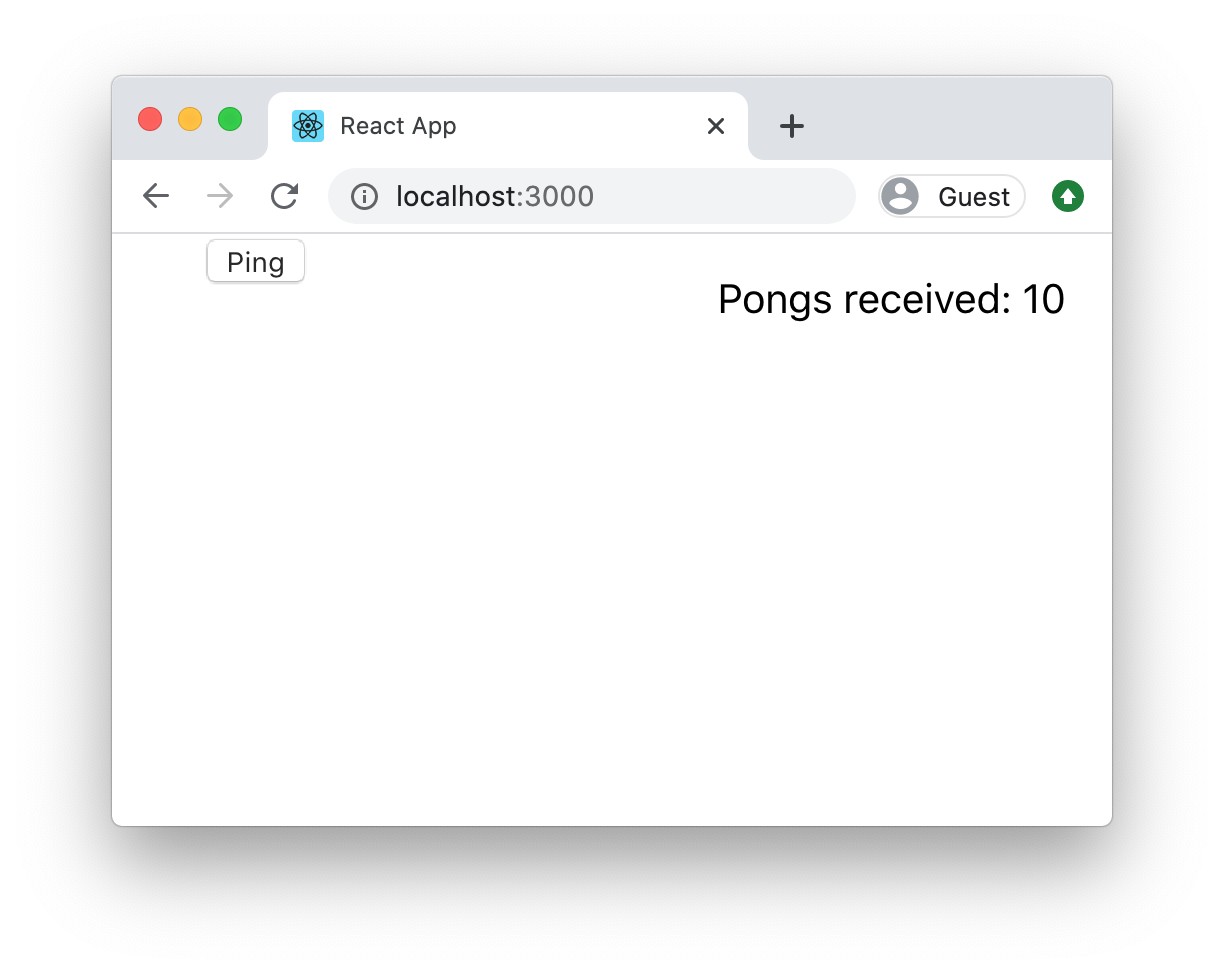
\includegraphics[width=0.5\textwidth]{pingpongclient}
\captionof{figure}{User interface of Ping Pong \trole{Client}}
\label{fig:pingpongclient}
\end{figure}

\subparagraph{Ping Pong \trole{Client} on React:}
\begin{itemize}

\item All \trole{Client}s implement the same user interface 
(\cref{fig:pingpongclient}), rendering
a \texttt{<button>} which triggers the send, and
a \texttt{<div>} captioned with the number of \tmsg{PONG}s received.

\item \trole{Client}s will use the React Context API \cite{reactcontext}
for application state management, i.e. the number of \tmsg{PONG}s received. 
We wrap the session logic in a \texttt{<Benchmark>} component 
that acts as the \texttt{ContextProvider} using its component state.

\item To automate the benchmark, we use the React Refs API \cite{reactrefs}
to access the DOM \texttt{<button>} node programmatically, in order to
simulate the click event and send a \tmsg{PING} message upon establishing
the WebSocket connection, or upon receiving a \tmsg{PONG}.

\item We use the production build generated by 
\texttt{create-react-app} \cite{cra} for all experiments, which performs the
transpilation into JavaScript. We serve the production build using the
\texttt{serve} package \cite{npmserve} available on \texttt{npm}.

\end{itemize}

\subparagraph{Ping Pong \trole{Svr} on Node:}
\begin{itemize}

\item We use the built-in \texttt{console.time} function to record
the execution time of all experiments. 
The timer starts when a WebSocket connection has been established at
\trole{Server}, and stops when on a \texttt{CloseEvent}.

\item To observe the execution pattern, the \trole{Svr} will log the running 
elapsed time for every \tmsg{PING} message received.

\item All \trole{Svr}s run the benchmarks without a real web browser,
using headless browsing functionality from 
the Zombie.js \cite{zombie} package.

\item \trole{Svr} logic is parameterised by the number of round trips,
$n$, configured through an environment variable passed through 
the command line.

\item We use the transpiled JavaScript versions of all \trole{Svr}s
for the experiments.

\end{itemize}

The interested reader may follow the instructions under
\texttt{benchmarks/README.md} in the project repository \cite{repo}
to run the benchmarks and visualise the logs using the interactive
notebook in the same directory.

We run the experiments under a network of latency 0.165ms
(64 bytes ping), and repeat each experiment 20 times.
Execution time measurements  are taken using a machine 
equipped with Intel i7-4850HQ CPU (2.3 GHz, 4 cores, 8 threads), 
16 GB RAM, macOS operating system version 10.15.4, 
Node.js runtime version 12.12.0, and
TypeScript compiler version 3.7.4.
We standardise all packages used in the front- and back-end
implementations across experiments. Details can be found in their
corresponding \texttt{package.json} manifests (\cref{appendix:eval}).

The benchmark compares three implementations of the Ping Pong protocol:

\subparagraph{bare:}
The \texttt{bare} implementation directly interfaces with 
WebSocket primitives for sending and receiving. 
The implementation executes the Ping Pong protocol, but does not 
guarantee communication safety by construction -- e.g. the user can click
the \tmsg{PING} button multiple times before a \tmsg{PONG} message 
is received, violating channel linearity. 
This represents the typical developer implementation without using the
MPST framework.

\subparagraph{bare_safe:}
The \texttt{bare_safe} implementation also directly interfaces with
WebSocket primitives for communication, but assumes the developer
implements minimal viable workarounds to address the lack of
communication safety. Here, the developer renders an inactive version
of the \tmsg{PING} button when the \tmsg{PING} message has been sent
but a response has yet to be received; a \texttt{visible} boolean flag
is used to explicitly manage which \texttt{<button>} to render.

\subparagraph{mpst:}
The \texttt{mpst} implementation uses the APIs generated from 
\fancyname{SessionTS}, so it enjoys the
communication safety guarantees from our methodology.

\subsection{Execution Pattern}
\label{section:execpattern}

We compare the execution patterns of exchanging 10,000 Ping-Pongs
throughout 20 repeated experiments across the three implementations.
We visualise the elapsed time with respect to the number of \tmsg{PING}s
received in \cref{fig:execution}.

\begin{figure}[!ht]
\centering
\begin{subfigure}[b]{0.3\textwidth}
\centering
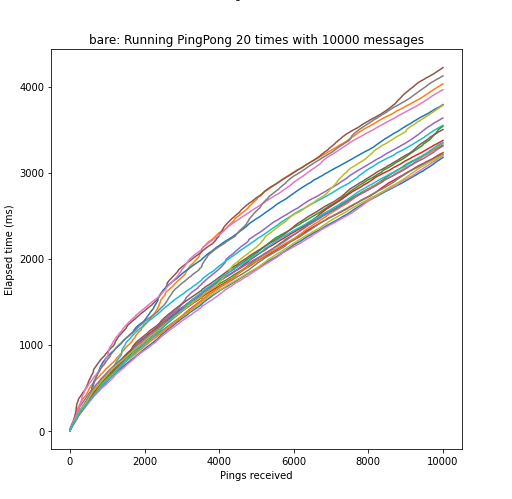
\includegraphics[width=\textwidth]{execbare10000}
\caption{\texttt{bare}}
\label{fig:executionbare}
\end{subfigure}
\hfill
\begin{subfigure}[b]{0.3\textwidth}
\centering
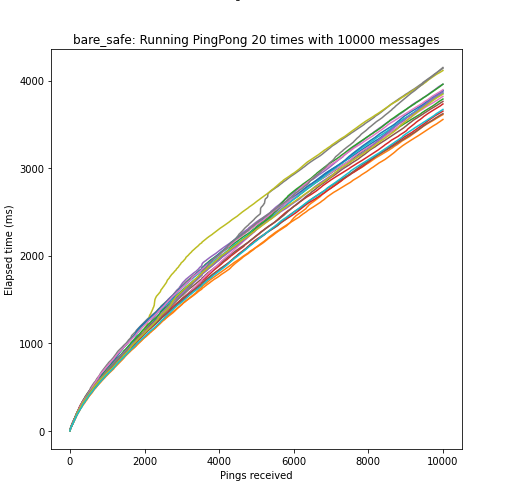
\includegraphics[width=\textwidth]{execbaresafe10000}
\caption{\texttt{bare_safe}}
\label{fig:executionbaresafe}
\end{subfigure}
\hfill
\begin{subfigure}[b]{0.3\textwidth}
\centering
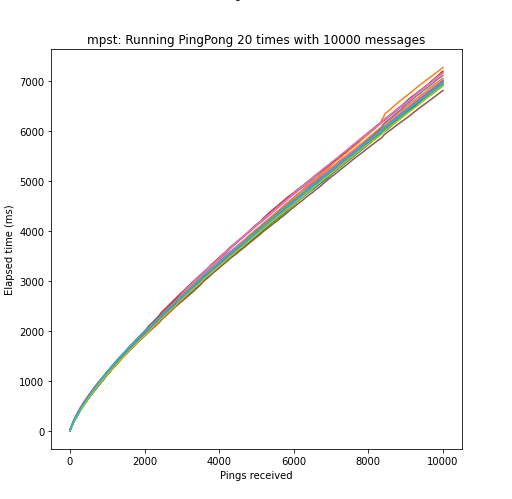
\includegraphics[width=\textwidth]{execmpst10000}
\caption{\texttt{mpst}}
\label{fig:executionmpst}
\end{subfigure}
\captionof{figure}{Comparison of Execution Pattern for 10,000 Ping-Pongs}
\label{fig:execution}
\end{figure}

Relative to the two \texttt{bare} implementations, the
\texttt{mpst} version performs more consistently, perhaps as a result
of the session runtimes handling all WebSocket interactions in a
systematic way. The gradient of the graph represents the rate at which
a Ping-Pong round trip takes place. 
We observe a steeper gradient when the protocol begins, 
which illustrates the overhead incurred in the 
session joining phase in our generated APIs.
Aside from these factors, all three implementations generally share
similar characteristics in their protocol execution.

\subsection{Overhead}
We compare the total execution time (\textit{Exec. Time}) 
and execution time per round trip (\textit{Exec. Time / Ping-Pong}) -- 
averaged over 20 repeated experiments -- across the three implementations,
for $n \in \{10^2, 10^3, 10^4\}$.
We summarise the results in \cref{table:overhead}.

\renewcommand{\arraystretch}{1.5}
\begin{table}[!ht]
\centering
\begin{tabular}{||c||c|c|c||c|c|c||}
\hline
\multirow{2}{*}{$n$} & 
\multicolumn{3}{c||}{Exec. Time} & 
\multicolumn{3}{c||}{Exec. Time / Ping-Pong} \\
\cline{2-7}
 & \texttt{bare} & \texttt{bare_safe} & \texttt{mpst} 
 & \texttt{bare} & \texttt{bare_safe} & \texttt{mpst} \\
\hline\hline
$10^2$ & 89.64ms & 107.09ms & 186.23ms & 0.90ms & 1.07ms & 1.86ms \\
$10^3$ & 642.92ms & 663.91ms & 1155.48ms & 0.64ms & 0.66ms & 1.16ms \\
$10^4$ & 3542.16ms & 3837.97ms & 7015.25ms & 0.35ms & 0.38ms & 0.70ms \\
\hline
\end{tabular}
\captionof{table}{Comparison of Execution Time for 
100, 1,000 and 10,000 Ping-Pongs}
\label{table:overhead}
\end{table}
\renewcommand{\arraystretch}{1}

We note that the addition of a session runtime for all roles in the 
\texttt{mpst} implementation \textit{does} incur a performance overhead. 
This is made apparent when looking closely at 
\textit{Exe. Time / Ping-Pong};
we visualise this in \cref{fig:timepermsg}.

\begin{figure}[!ht]
\centering
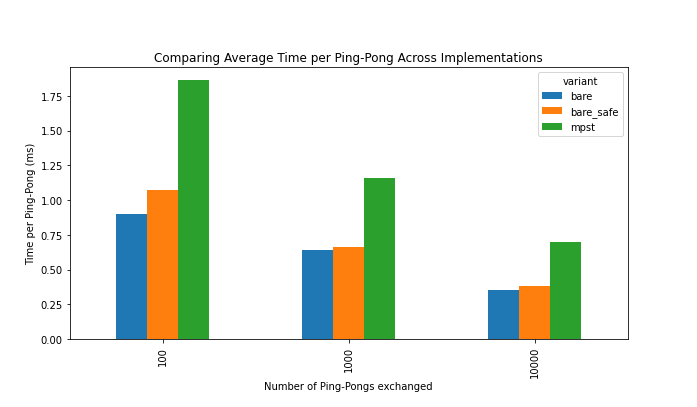
\includegraphics[width=\textwidth]{timepermsg}
\captionof{figure}{Comparing Average Time per Ping-Pong 
Across Implementations}
\label{fig:timepermsg}
\end{figure}

The \texttt{mpst} implementation records greater round trip times compared
to both \texttt{bare} and \texttt{bare_safe} variants. This is expected,
as the runtime for \textit{each} role performs additional logic during
\textit{both} the sending and receiving of messages. 
For example, receiving a message involves performing
(albeit $O(1)$ time complexity) operations on the message queue and
handler queue. As for browser-side implementations, every EFSM transition
invokes an updated \texttt{render()} on the VDOM, which requires
reconciliation internally by React to update the browser DOM accordingly.

We also observe that the (round trip time) performance gap between 
the \texttt{mpst} implementation and the two 
\texttt{bare} implementations narrows as the number of round trips 
increase. This suggests that the session joining logic in our
implementation yields greater overhead than the additional processing
logic injected during communication, which is consistent with 
our findings in \cref{section:execpattern}.

We interpret the overhead as a trade-off between maximising performance and
maximising the \textbf{static} communication safety guarantees for
web applications. In particular, the event-driven nature of 
browser-side logic makes it highly challenging to guarantee 
communication safety, as having ``active'' channel actions on the DOM
allows linearity to be violated by the user, even if one verifies
linear channel usage in the source code. The \texttt{mpst} implementation
properly addresses the problem by statically guaranteeing,
by construction, that the UI component rendered on the DOM will only
contain channel actions permitted at that state in the EFSM execution.

One may argue that the \texttt{bare_safe} implementation also
provides said guarantee but adds negligible overhead. 
By inspecting the workaround in the \texttt{bare_safe} implementation
(\cref{lst:workaround}),
it is clear that this does not scale for more complicated protocols with
larger EFSMs. 

\begin{figure}[!ht]
\begin{lstlisting}[language=javascript, tabsize=2]
click() {
	this.state.ws?.send(JSON.stringify({
		label: 'PING',
		payload: [this.context.count],
	}));
	this.setState({ visible: false });
}

render() {
	return this.state.visible 
		? <button
		   ref={this.state.button}
		   onClick={this.click.bind(this)}
		   >Ping</button>
		: <button>Ping</button>;
}
\end{lstlisting}
\captionof{lstlisting}{Preventing user-triggered linearity violation in
\texttt{bare_safe} Ping Pong}
\label{lst:workaround}
\end{figure}

The workaround is tailored to the Ping Pong protocol
and toggles the \texttt{visible} flag to hide the button that triggers
a send action when \trole{Client} transitions to a receive state.
In fact, this ``workaround'' precisely generalises to our 
\texttt{mpst} implementation of having some form of wrapper
component that renders the UI component corresponding to the
current EFSM state. Our API generation strategy formally implements
the EFSM for browser-side logic.

We also compare the server-side logic between the \texttt{base} and
\texttt{mpst} implementations in \cref{fig:nodepingpong}, and observe
that our generated APIs (\cref{lst:nodepingpongmpst}) 
allow the developer to focus on the
implementation detail, whilst the naive bare implementation 
(\cref{lst:nodepingpongbare}) chooses to interleave communication logic
with application logic, which arguably contributes towards a hidden
source of bugs found when implementing more complex protocols.

\begin{figure}[!ht]
\centering
\begin{subfigure}[b]{\textwidth}
\centering
\begin{lstlisting}[language=javascript,tabsize=2]
socket.onmessage = ({ data }) => {
	const { label, payload } = JSON.parse(data.toString());
	if (label === 'PING') {
		let count: number = payload[0];
		console.timeLog(LABEL, ++count);
		if (count === MSGS) {
			socket.send(JSON.stringify({
				label: 'BYE',
				payload: [count],
			}));
		} else {
			socket.send(JSON.stringify({
				label: 'PONG',
				payload: [count],
			}));
		}
	} else {
		throw new Error(`Unrecognised label: ${label}`);
	}
}
\end{lstlisting}
\caption{\texttt{bare} implementation of Ping Pong \trole{Svr}}
\label{lst:nodepingpongbare}
\end{subfigure}
\hfill
\begin{subfigure}[b]{\textwidth}
\centering
\begin{lstlisting}[language=javascript,tabsize=2]
// NOTE: `Implementation' namespace omitted for brevity.

const logic = new S14({
	PING: (count) => {
		console.timeLog(LABEL, ++count);
		if (count === MSGS) {
			return new S16([Labels.S16.BYE, [count], new S15()]);
		} else {
			return new S16([Labels.S16.PONG, [count], logic]);
		}
 	}
});
\end{lstlisting}
\caption{\texttt{mpst} implementation of Ping Pong \trole{Svr}}
\label{lst:nodepingpongmpst}
\end{subfigure}
\captionof{figure}{Comparison of \texttt{bare} and \texttt{mpst}
implementations for Ping Pong \trole{Svr}}
\label{fig:nodepingpong}
\end{figure}